\section{Phonons in Three Dimensions}
% Logistics - MT on Nov. 2nd. Short in-class exam of 15-20 minutes of a few simple questions that everyone should know how to do. There is a practice MT. Takehome will be 3 problems, have until Nov. 7th to complete.
% Topics - We will finish phonons today, then discuss magnetic structure and magnons, then electrons in periodic potential and band structure theory. This will be the extent of the content covered.
\subsection{Review - The Real and Reciprocal 3D Lattice}
We consider atoms located at positions $\v{R}$ of a Bravais lattice in 3D space. Such a Bravais lattice can be written via:
\begin{equation}
    \v{R} = n_1\v{a}_1 + n_2\v{a}_2 + n_3\v{a}_3
\end{equation}
where $n_i \in \ZZ$ and $\v{a}_i$ are primitive vectors.

The corresponding reciprocal lattice vectors $\v{G}$ are defined by $e^{i\v{R} \cdot \v{G}} = 1$, which implies:
\begin{equation}
    \v{G} = m_1 \v{b}_1 + m_2\v{b}_2 + m_3\v{b}_3.
\end{equation}
Where $m_j \in \ZZ$ and $\v{b}_j$ are primitive vectors of the reciprocal lattice, satisfying the usual relation:
\begin{equation}
    \v{a}_i \cdot \v{b}_j = 2\pi \delta_{ij}.
\end{equation}

We will also need a relation:
\begin{equation}
    \sum_{\v{R}}e^{i\v{R} \cdot \v{q}} = N\sum_{\v{G}}\delta_{q\v{G}} = N\Delta (\v{q})
\end{equation}

\subsection{Writing down the 3D Hamiltonian}
The Hamiltonian for the 3d lattice with the harmonic approximation can be written as:
\begin{equation}
    H = \sum_{\v{R}, i}\frac{(p^i_\v{R})^2}{2M} + \frac{1}{2}\sum_{\v{R}, \v{R}'}\mu^i_\v{R} V_{\v{R}\v{R}'}^{ij}\mu^j_{\v{R}'}
\end{equation}
This is the expected generalization from 1D, where we see that the atoms can move and vibrate in three dimensions; $i, j \in \set{x,y,z}$. $V^{ij}_{\v{R}\v{R}'}$ (as before) is the dynamical matrix $V_{\v{R}\v{R'}}^{ij} = \left.\frac{\partial^2 V}{\partial \mu_\v{R}^i \partial \mu_{\v{R}'}^j} \right|_{\gv{\mu} = 0}$. We define the displacement/momenta at each lattice site as:
\begin{equation}
    \begin{split}
        \v{Y}_\v{R} &= \m{\mu_\v{R}^x \\ \mu_\v{R}^y \\ \mu_{\v{R}}^z}
        \\ \v{P}_\v{R} &= \m{p_\v{R}^x \\ p_\v{R}^y \\ p_{\v{R}}^z}
    \end{split}
\end{equation}
And therefore the Hamiltonian becomes:
\begin{equation}
    H = \frac{1}{2M}\sum_\v{R}\v{P}^T_\v{R} \v{P}_\v{R} + \frac{1}{2}\sum_{\v{R},\v{R}'}\v{Y}^T_\v{R} \m{V_{\v{R}\v{R}'}^{xx} & V_{\v{R}\v{R}'}^{xy} & V_{\v{R}\v{R}'}^{xz} \\ V_{\v{R}\v{R}'}^{yx} & V_{\v{R}\v{R}'}^{yy} & V_{\v{R}\v{R}'}^{yz} \\ V_{\v{R}\v{R}'}^{zx} & V_{\v{R}\v{R}'}^{zy} & V_{\v{R}\v{R}'}^{zz}} \v{Y}_{\v{R}}
\end{equation}
note that due to the definition of the dynamical matrix elements, the matrix appearing in the above expression is a real symmetric matrix.

\subsection{Translation Invariant Solution}
With the assumption of translation invariance, we obtain the condition $V^{ij}_{\v{R}\v{R}'} = V^{ij}_{\v{R} - \v{R}'}$. As we did for the 1D case, we will use a fourier transform:
\begin{equation}
    \v{Y}_\v{q} = \frac{1}{\sqrt{N}}\sum_{\v{R}}e^{-i\v{q} \cdot \v{R}}Y_\v{R}, \quad \v{P}_\v{q} = \frac{1}{\sqrt{N}}\sum_\v{R}e^{i\v{q} \cdot \v{R}}\v{P}_{\v{R}}
\end{equation}
As in 1D, we also have the periodicity:
\begin{equation}
    \v{Y}_{\v{q} + \v{G}} = \v{Y}_{\v{q}}, \quad \v{P}_{\v{q} + \v{G}} = \v{P}_\v{q}
\end{equation}
This defines the 3D Brillouin zone $\mathcal{B}$ as the fundamental domain of $\v{q}$. The Inverse FT gives:
\begin{equation}
    \v{Y}_\v{R} = \frac{1}{\sqrt{N}}\sum_{\v{q} \in \mathcal{B}}e^{i\v{q} \cdot \v{R}}\v{Y}_\v{q}, \quad \v{P}_\v{R} = \frac{1}{\sqrt{N}}\sum_{\v{q} \in \mathcal{B}}e^{-i\v{q} \cdot \v{R}}\v{P}_\v{q}
\end{equation}
The Hamiltonian reduces to:
\begin{equation}
    H = \sum_{\v{q} \in \mathcal{B}} \left(\frac{1}{2M}\v{P}^\dag_\v{q} \v{P}_\v{q} + \frac{1}{2}\v{Y}_q^\dag \m{V_{\v{q}}^{xx} & V_{\v{q}}^{xy} & V_{\v{q}}^{xz} \\ V_{\v{q}}^{yx} & V_{\v{q}}^{yy} & V_{\v{q}}^{yz} \\ V_{\v{q}}^{zx} & V_{\v{q}}^{zy} & V_{\v{q}}^{zz}}\v{Y}_\v{q}\right)
\end{equation}
where the $3N \times 3N$ matrix in the original basis has now reduced to a $3 \times 3$ matrix. The matrix elements in this basis are:
\begin{align*}
    \v{V}_{\v{q}}^{ij} = \sum_{\v{R}'}e^{i\v{q} \cdot (\v{R} - \v{R}')}V_{\v{R}\v{R}'}^{ij}
\end{align*}
To complete this solution, we have to diagonalize the $3 \times 3$ dynamical matrix. It is a Hermitian matrix and thus has three orthogonal vectors $\v{s}_1, \v{s}_2, \v{s}_3$ belonging to eigenvalues $\v{v}^1_\v{q}, \v{v}^2_\v{q}, \v{v}^3_\v{q}$. In this basis defined by these three orthogonal vectors, we have:
\begin{equation}
    H = \sum_{\v{q}, \mu=1,2,3}\left(\frac{p_q^{\mu\dag}p_q^\mu}{2M} + \frac{1}{2}V_q^\mu \mu_q^{\mu^\dag}\mu^\mu_q\right)
\end{equation}
where $\mu_q^\mu = \gv{\mu}_\v{q} \cdot \v{s}_\mu$ and $p_q^\mu = \v{p}_\v{q} \cdot \v{s}_\mu$. 

The 3 directions described by $\v{s}_\mu(\v{q})$ define phonon \emph{polarization}. In addition, for $\v{q}$ along a high-symmetry axis, we typically have $\v{s} \parallel \v{q}$ which is a ``longitudinal phonon'' and $\v{s} \perp \v{q}$ which is two ``transverse phonons''.

Why a high symmetry axis? If we take an arbitrary $\v{q}$ pointing in some random direction in reciprocal space, in general none of the $\v{s}$ will be parallel to $\v{q}$ or orthogonal to it. But when the phonon propogates along a high symmetry axis, we do typically see this separation.

Phonon frequencies are given by:
\begin{equation}
    \omega_{\v{q}\mu} = \sqrt{\frac{V_\v{q}^\mu}{M}}
\end{equation}
and the corresponding raising/lowering operators are:
\begin{equation}
    a_{\v{q}\mu} = \frac{1}{\sqrt{2M\hbar \omega_{\v{q}\mu}}}(M\omega_{\v{q}\mu}\mu^\mu_\v{q} + ip_\v{q}^{\mu\dag}), \quad a_{\v{q}\mu}^\dag = \ldots
\end{equation}
which leads to:
\begin{equation}
    H = \sum_{\v{q}, \mu}\hbar \omega_{\v{q}\mu}(a^{\dag}_{\v{q}\mu}a_{\v{q}\mu} + \frac{1}{2})
\end{equation}

One more comment before moving onto the next topic; this was all for a simple Bravais lattice. This is the simplest possible type of crystal structure where you have one type of atom periodically repeating in space. Most solids are not quite so simple and have a larger unit cell, such as Sodium Chloride. Things would work out exactly the same in this case, there would just be an additional index labelling the position of the atom inside the unit cell (of which there are $n_b$). The $3 \times 3$ matrix would become a larger $3n_b \times 3n_b$ matrix with $3n_b$ eigenvalues/eigenvectors, which describe the internal degrees of freedom in the unit cell. Previously, we had 3 polarizations for the one atom type. Now we have 3 polarizations per atom type, so there is a more complex structure with more modes (e.g. different atoms can vibrate in different directions). Of these, 3 will be acoustic modes (frequency goes to zero as $\v{q} \to \v{0}/\lambda \to \infty$), and $3(n_b - 1)$ will be acoustic modes.

\begin{figure}[htbp]
    \centering
    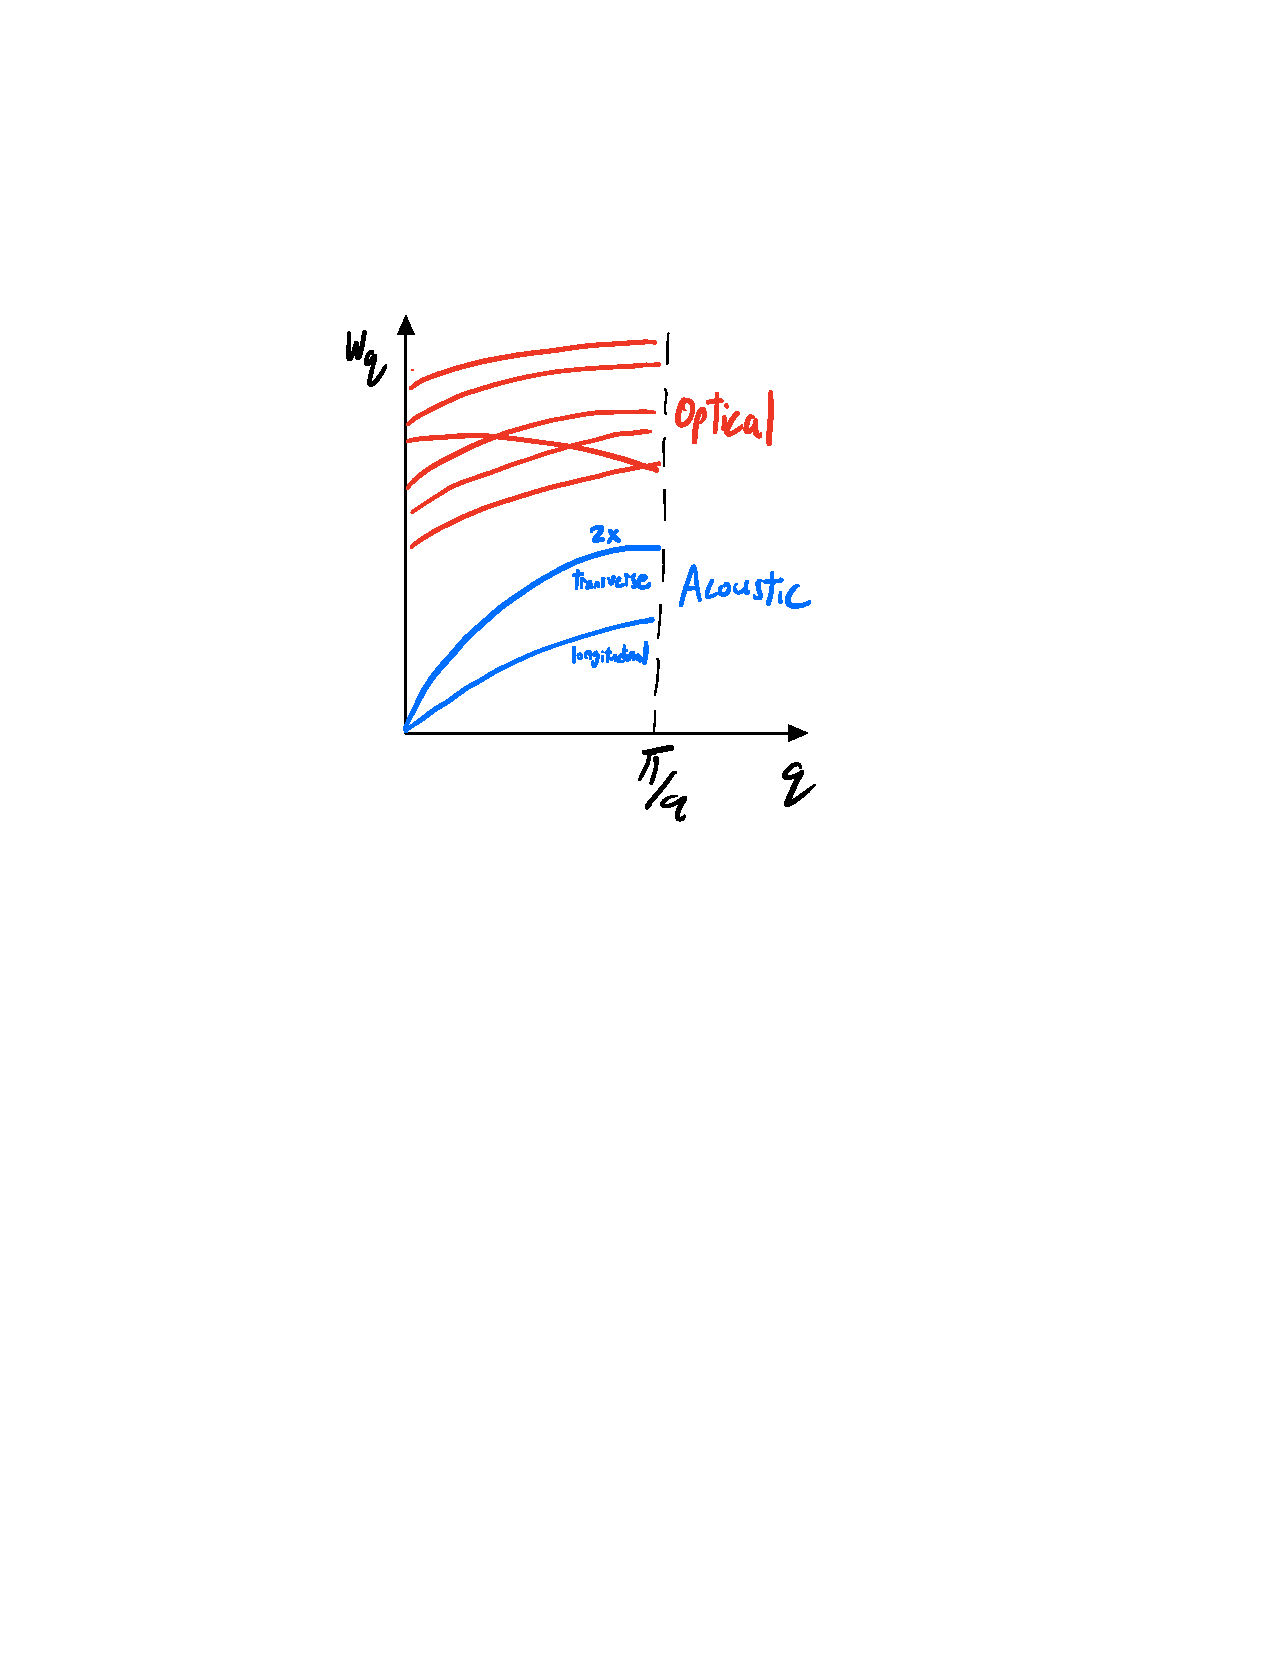
\includegraphics[scale=0.7]{Images/fig-3dphonondispersion.pdf}

    \caption{Plot of the phonon dispersion curves for a complex 3d solid. We have 3 acoustic modes (1 longitudinal mode and 2 degenerate transverse modes) and $3(n_d - 1)$ optical modes. }
    \label{fig-3dphonondispersion}
\end{figure}

\subsection{Debye Model, Specific Heat of Phonons}
This was one of the main puzzles in solid-state physics before the advent of QM! Let's figure out how to calculate this. The internal energy in lattice vibrations is given by:
\begin{equation}
    U = \avg{H}_\beta = \sum_{\v{q}\mu}\hbar \omega_{\v{q}\mu}(\avg{a^\dag_{\v{q}\mu}a_{\v{q}\mu}} + \frac{1}{2})
\end{equation}
Where $\avg{a^\dag_{\v{q}\mu}a_{\v{q}\mu}} = \bar{n}_{\v{q}\mu} = \frac{1}{e^{\beta \hbar \omega_{\v{q}\mu}} - 1}$ is the bose-einstein occupation factor. It will actually be easier to go straight to the heat capacity:
\begin{equation}\label{eq-photonCV}
    C_V = \dod{U}{T} = \frac{1}{k_B T^2}\sum_{\v{q}, \mu}\frac{(\hbar \omega_{\v{q}\mu})^2 e^{\beta \hbar \omega_{\v{q}\mu}}}{(e^{\beta\hbar\omega_{\v{q}\mu}} - 1)^2}
\end{equation}
to evaluate the sum we would need to know the form of $\omega_{\v{q}\mu}$, and even then there usually does not exist a closed-form solution for the summation.

To evaluate Eq. \eqref{eq-photonCV}, it is useful to define the phonon density of states:
\begin{equation}
    D(\omega) = \sum_{\v{q}, \mu} \delta(\omega - \omega_{\v{q}\mu})
\end{equation}
This implies:
\begin{equation}
    C_V = \frac{1}{k_BT}\int_0^\infty d\omega D(\omega)\frac{(\hbar\omega)^2 e^{\beta\hbar\omega}}{(e^{\beta\hbar\omega} - 1)^2}
\end{equation}
The Debye model assumes $\omega_{\v{q}\mu} = c_\mu\abs{\v{q}}$, approximating the acoustic modes as straight lines. It should be accurate at low $T$ when only low frequency acoustic phonons are thermally excited. For simplicity, we further assume equal velocities $c_\mu = c$ for $\mu = 1,2,3$ (but this is not essential, and the calculation can still be done). We then get:
\begin{equation}
    \begin{split}
        D(\omega) &= \frac{3V}{(2\pi)^3}\int d^3q \delta(\omega - cq)
        \\ &= \frac{3V}{(2\pi)^3}4\pi \int q^2 dq \delta(\omega - cq) 
        \\ &= \frac{3V}{3\pi^2}\frac{\omega^2}{c^3}.
    \end{split}
\end{equation}
where the $3$ comes from the 3 directions summed over and we evaluate the integral by going into spherical coordinates. 

\subsection{Debye Frequency, Momentum, Temperature}
There is one more constraint for us to accomodate. The density of states has the property that if we integrate over it, we should get the total number of modes in the entire system (which in this case should be $3N$; $N$ particles moving in three dimensions). Therefore, the above expression cannot go on forever; and this is evident from the acoustic spectra where we see there are no states above some energy. So, we introduce a Debye frequency $\omega_D$:
\begin{equation}
    D(\omega) = \begin{cases}
        \frac{3V}{2\pi^2}\frac{\omega^2}{c^3} & \Omega < \omega_D
        \\ 0 & \omega > \omega_D
    \end{cases}
\end{equation}
where $\omega_D$ is determined by:
\begin{equation}
    \int_0^{\omega_D}D(\omega)d\omega = 3N \implies \omega_D^3 = 4\pi^2c^3\frac{N}{V}
\end{equation}'

\begin{figure}[htbp]
    \centering
    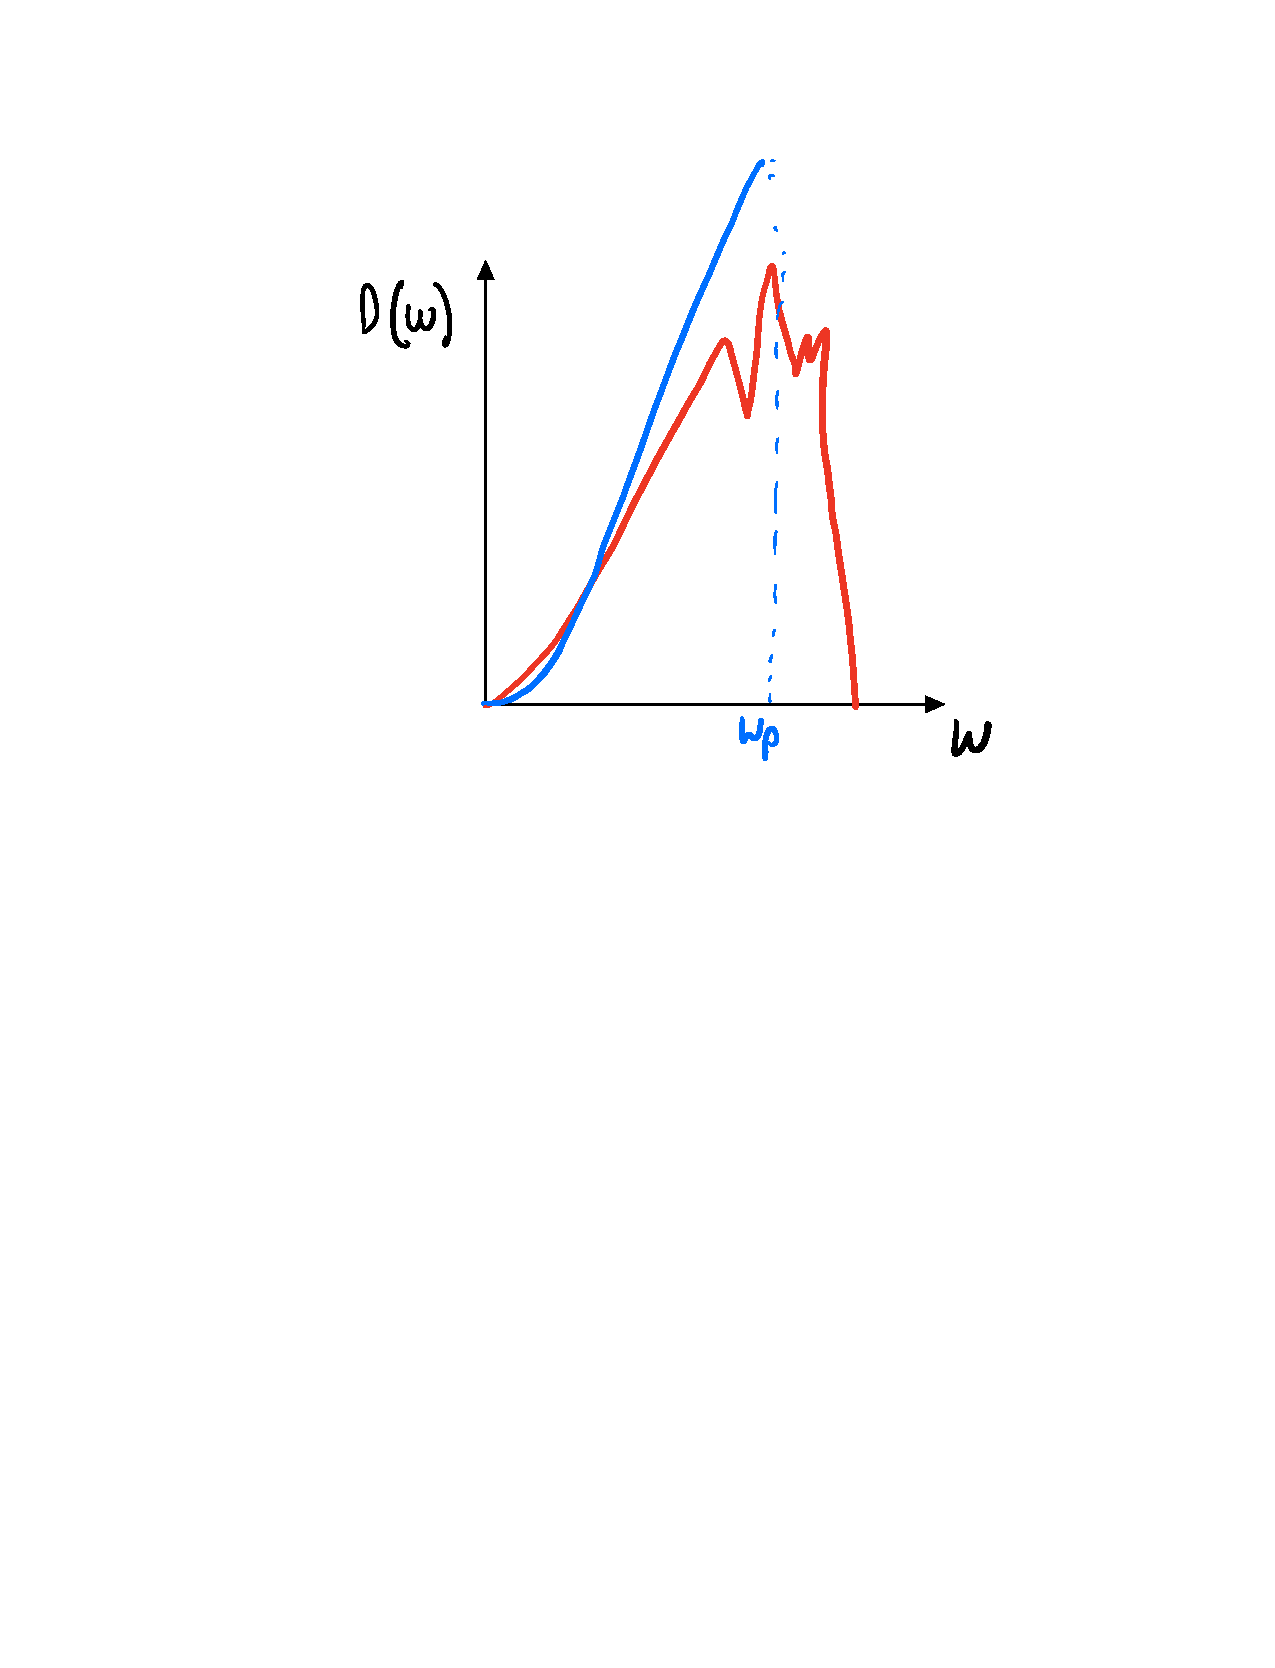
\includegraphics[scale=0.6]{Images/fig-phonondensityofstates.pdf}

    \caption{Plot of a realistic/experimentally measured phonon density of states (red) and our approximate calculated value (blue). We cut off the $\omega^2$ prediction for the density of the states at the Debye frequency $\omega_D$ such that the area under the curve (i.e. the total number of modes) is $3N$ (and the same for the two plots). It may seem like we neglect a lot of structure in making our approximation, but since we are itnerested in the heat capacity $C_V$, this complex structure generally gets smeared out regardless; hence our approximation can give reasonable predictions for heat capacity.}
    \label{fig-phonondensityofstates}
\end{figure}

This notion of a Debye frequency turns out to be very useful. It also defines Debye momentum:
\begin{equation}
    k_D = \frac{\omega_D}{c} = \left(6\pi^2\frac{N}{V}\right) \sim \frac{4}{a}
\end{equation}
where $a$ is the lattice spacing. It also defines the Debye temperature:
\begin{equation}
    \Theta_D = \frac{\hbar\omega_D}{k_B} \sim 74\si{K} - 1800\si{K}
\end{equation}
where $74\si{K}$ corresponds to Pr and $1800\si{K}$ corresponds to diamond. On average it is on the order of a few hundred Kelvin. These are all characteristic scales of phonons. Of all of them, Debye temperature tends to be the most useful as it is in the most tangible units. It distinguishes a low and high temperature regime for phonon excitations (i.e. the frequency for which below it the acoustic approximation is reasonable)

\subsection{Back to Heat Capacity}
We have:
\begin{equation}
    \begin{split}
        C_V &= \frac{3V\hbar^2}{2\pi^2c^2k_BT^2}\int_0^{\omega_B}d\omega \frac{\omega^4 e^{\beta\hbar\omega}}{(e^{\beta\bar\omega} - 1)^2}
        \\ &= gNk_B\left(\frac{T}{\theta_D}\right)^3\int_0^{\theta_D/T} dx \frac{x^4e^x}{(e^x - 1)^2}
    \end{split}
\end{equation}
where we have made the substitution $x = \beta\hbar\omega$. We call the integral $f(\theta_D/T)$ the Debye function.

